\documentclass[a4paper, fontsize=12pt, ngerman, oneside, openright]{scrreprt}

% Rendering packages
\usepackage{amsmath}
\usepackage{amssymb}
%\usepackage[draft]{graphicx}
\usepackage{graphicx}
\usepackage{wrapfig}
\usepackage{svg}
\usepackage{subcaption}
\usepackage{placeins}
\usepackage{xcolor}      % use if color is used in text
\usepackage{eurosym}


% Page dimensions
\usepackage[inner=2.5cm,outer=2.5cm,top=3.7cm,bottom=3.5cm]{geometry} 
\usepackage{parskip}
\usepackage[onehalfspacing]{setspace}

% Font styling
\usepackage[english]{babel}
\usepackage[utf8]{inputenc}
\usepackage[T1]{fontenc}
\usepackage{lmodern}
\renewcommand\familydefault{\sfdefault}
\usepackage[11pt]{moresize}

% Tables
\usepackage{tabularx}
\usepackage{tabulary}
\usepackage{longtable, lscape}

% Headers
\usepackage{scrpage2}  % header and footer for KOMA-Script
\pagestyle{scrheadings}
\automark[section]{chapter}

% Zitate
\usepackage[backend=biber, 
			style=authoryear,
			isbn=false, 
			sorting=nyt,
			]{biblatex}
\usepackage[babel,german=quotes, english=british, threshold=3]{csquotes}
\bibliography{Bibliothek/Bibliothek}

\usepackage[hyperindex,breaklinks,colorlinks=true,linkcolor=black,urlcolor=blue,citecolor=black]{hyperref}

% Code Blöcke
\usepackage{listings}
%\usepackage{Header/listings-golang} % import this package after listings
\usepackage{syntax}



%\lstset{ % add your own preferences
%	frame=single,
%	captionpos=b,
%	mathescape=true,
%	basicstyle=\footnotesize\ttfamily,
%	keywordstyle=\color{black},
%	numbers=left,
%	numbersep=5pt,
%	showstringspaces=false, 
%	stringstyle=\color{blue},
%	tabsize=2,
%	language=Golang % this is it !
%}


%table colors
\usepackage{xcolor,colortbl}

\newcommand{\mc}[2]{\multicolumn{#1}{c}{#2}}
\definecolor{Gray}{gray}{0.85}
\definecolor{LightCyan}{rgb}{0.88,1,1}

\newcolumntype{a}{>{\columncolor{Gray}}c}
\newcolumntype{b}{>{\columncolor{Gray}}l}

\usepackage{color}
\definecolor{gray}{rgb}{0.4,0.4,0.4}
\definecolor{darkblue}{rgb}{0.0,0.0,0.6}
\definecolor{cyan}{rgb}{0.0,0.6,0.6}
\definecolor{dkgreen}{rgb}{0,0.6,0}
\definecolor{gray}{rgb}{0.5,0.5,0.5}
\definecolor{mauve}{rgb}{0.58,0,0.82}

\lstset{
  basicstyle=\ttfamily,
  columns=fullflexible,
  showstringspaces=false,
  commentstyle=\color{gray}\upshape
}

\lstset{
	frame=tb,
	language=Java,
	aboveskip=3mm,
	belowskip=3mm,
	showstringspaces=false,
	columns=flexible,
	basicstyle={\small\ttfamily},
	numbers=none,
	numberstyle=\tiny\color{gray},
	keywordstyle=\color{blue},
	commentstyle=\color{dkgreen},
	stringstyle=\color{mauve},
	breaklines=true,
	breakatwhitespace=true,
	tabsize=3,
	numbers=left
}

\lstdefinelanguage{XML}
{
	morestring=[b]",
	morestring=[s]{>}{<},
	morecomment=[s]{<?}{?>},
	morecomment=[s]{!--}{--},
	stringstyle=\color{black},
	identifierstyle=\color{darkblue},
	keywordstyle=\color{cyan} list your attributes here
}

%pdf insert
\usepackage{pdfpages}

%zusätzliche Trennungen
\hyphenation{Grund-ar-chi-tek-tur}
\hyphenation{MQTT-Kom-mu-ni-ka-tions-mo-dell}
\hyphenation{Master-Master-Replikation}
\hyphenation{Pub-lish-er}
\hyphenation{Pub-lish-ers}
\hyphenation{Sub-scriber}
\hyphenation{Sub-scribers}
\hyphenation{Pub-lish er/Sub-scriber}
\hyphenation{beo-bacht-bar}
\hyphenation{Score}
\hyphenation{Ac-knowl-edge-ment}
\hyphenation{Ac-knowl-edge-ments}

\usepackage{mathtools}
\DeclarePairedDelimiter\abs{\lvert}{\rvert}

\usepackage{acronym}



\begin{document}

% Titelseite einfügen.
\begin{titlepage}


\begin{center}
 		
\includegraphics[scale=0.3]{Resources/Logo3}
\end{center}

\begin{center}
	\HUGE \textbf{Varroa}
	\large\\MQTT-Scenario-Testing-Tool\\ \ \\
	\small Masters Level Study Project, Prof. PhD. Siebert \\
	SS 2018 - WS 2018/2019
\end{center}

\begin{center}
R. Atherton, S. Baier, S. Giebl, G. Held, Y. Weber, T. Weiden
\end{center}

\end{titlepage}



% Counter zurücksetzen. Römische Ziffern einstellen.
\pagenumbering{Roman}
\setcounter{page}{1}

% Inhaltsverzeichnis generieren.
\tableofcontents

% Neue Seite. Counter zurücksetzen. Arabische Ziffern einstellen.
\pagenumbering{arabic}
\setcounter{page}{1}

% Kapitel einfügen.
\chapter{Vision}
The lack of testability of MQTT systems was the motivation for creating \emph{Varroa} -- a MQTT testing tool.
The name \emph{Varroa} is inspired by the varroa mite, which is a species of mite that infects honey bee colonies.
Figuratively our MQTT testing tool works in a similar way but instead of infesting a hive, it tries to infest a broker.
This association between the bee hives of the natural realm and those of the MQTT world came from the \emph{HiveMQ} MQTT broker's branding.


The basic use-case of \emph{Varroa} is testing the resilience of brokers by creating load.
To achieve this, \emph{Varroa} is able to simulate a large amount of MQTT clients by a simple and descriptive Scenario definition.
A Scenario can be easily declared by a domain specific language which is defined in a XSD file.


Furthermore Varroa can be executed as a distributed system.
If this is the case the workload is automatically split and distributed to different machines.
This enables great horizontal scaling potential.
In this context scaling means that the amount of MQTT clients can easily be increased.



\chapter{Concepts}
To understand the workings of Varroa, we will have to take a look at the different parts that make up the system.
Furthermore we explain the basic concepts of MQTT.

\section{Varroa Distributed System Concepts}
A Varroa Distributed System orchestration of multiple Varroa instances consisting of one Commander and at least one Agent.
Varroa is organized as a distributed system, due to the impossibility of creating enough MQTT-clients on a single machine to overload a MQTT-broker, especially if the broker is also a distributed system.

\paragraph{Varroa Instance}
A Varroa instance is a running Varroa process in a single JVM, can be either Commander or Agent.

\paragraph{Commander}
The Commander is a part of the Varroa Distributed System, that parses the scenario, generates chunks and distributes them to the Agents.
Only one Commander exists in a Varroa distributed system.

\paragraph{Agent}
The Agent is part of the Varroa Distributed System.
It receives Chunks from the Commander and passes them to its MQTT-Agents.
A Varroa distributed system contains at least one Agent.

\paragraph{MQTT Agent}
MQTT Agents are components of an Agent.
Every MQTT Agent manages one MQTT client.

\paragraph{Chunk}
The scenario is split in Chunks by the Commander and then those Chunk are distributed to the agents.
%A Chunk is a Collection of Information, such as which commands are to be sent to the broker as well as how many clients should perform these commands.
%Another important information, contained in the Chunk is at which rate these commands are to be executed.

%A scenario is a XML-Document which defines a sequence of stages.

\section{Varroa Scenario Concepts}
The integral idea of Varroa is testing scenarios, which means simulating the behaviour of a large amount of MQTT clients.
It tests whether the broker can handle the associated load.
A scenario is an abstract representation of a real MQTT-Use-Case.
It defines the topology of all participating MQTT clients and brokers.

\paragraph{MQTT Client}
A MQTT client is used to execute the Commands to create load.
Those clients implement the MQTT protocol using the HiveMQ MQTT Client.

\paragraph{Client Group}
Client groups are part of the scenario.
They enable the user to define the behaviour and properties of a group of MQTT clients with a configurable size.
These MQTT clients are created by Varroa for the purpose of simulating the MQTT clients of a scenario.
The lifespan of the spawned MQTT clients does not exceed the lifespan of a scenario.

\paragraph{Command}
A command is an abstract representation of a work step that must be executed by a MQTT client.

\paragraph{Topic Group}
A Topic Group represents a number of topics that share a naming pattern.
This concept enables the user to model the interaction between Client Groups and a number of similar topics.

\section{General MQTT Concepts}
\paragraph{Broker}
The Broker serves as an intermediary between publishers and subscribers.
It takes over the routing of the exchanged MQTT messages and is the central control authority of a MQTT Network.
%TODO cite Georg
\paragraph{Client}
A client that implements the MQTT protocol. 
\paragraph{Topic}
Topics are strings separated by slashes that do not contain wild-cards.
Messages published with Topic are delivered to subscribers that have registered matching Topic Filters.
\paragraph{Topic Filter}
A Topic Filter is a chain of strings delimited by slashes that 
can cover one or more topics. 
It can also contain wild-cards: a plus sign covers a single hierarchy level, a double cross selects all possible following levels.
\paragraph{Publisher}
Publishers are clients that produce data.
They send messages with a specific topic to the broker.
\paragraph{Subscriber}
Subscribers are clients that subscribe to a subset or to all messages sent via the
MQTT network.
They log on to the broker and register with one or more topic filters that specify the topics whose messages they want to receive.
%TODO cite Georg
\paragraph{Connect}
Disconnect describes the process of a Client establishing a connection to a Broker.
\paragraph{Disconnect}
Connect describes the process of a Client terminating its connection to a Broker.



\chapter{Scenario Concept}

%\begin{lstlisting}[caption={Implementierung des Trainierens der Markov-Chain}, captionpos=b, label={lst:train}, language=XML]
% <!-- -->
%\end{lstlisting}


\begin{lstlisting}[caption={XML definition of the Scenario}, captionpos=b, label={lst:scenario}, language=XML]
<scenario>
	<broker id="b1">
		<!-- definition broker parameters -->
	</broker>
	
	<clientGroups>
		<!-- definition of client groups -->
	</clientGroups>
	
	<topicGroups>
		<!-- definition of topic groups -->
	</topicGroups>
	
	<subscriptions>
		<!-- definition of subscriptions -->
	</subscriptions>

	<waitPatterns>
		<!-- definition of waitPatterns -->
	</waitPatterns>
	
	<stages>
		<!-- definition of stages -->
	</stages>
</scenario>
\end{lstlisting}

A Varroa test is the execution of a user defined Scenario, which is specified in a XML file.
To define a valid scenario the user needs to define the topology of the Scenario and the behaviour of its components.
An example for the outline of a Scenario XML file is given in \ref{lst:scenario}.

\section{Broker}
\begin{lstlisting}[caption={XML definition of the Broker}, captionpos=b, label={lst:broker}, language=XML]
<scenario>
	<broker id="b1">
		<address>broker.hivemq.com</address>
		<port>1883</port>
	</broker>
</broker>
\end{lstlisting}
The broker is the central component whose performance and stress resistance is tested by the Scenario.
For this the user needs to define:
\begin{itemize}
	\item \textbf{id:} the identifier to reference the broker.
	\item \textbf{address:} the address of the broker can either be a IPv4-Address or a Fully-Qualified-Domain-Name.
	\item \textbf{port:} the port on which the broker is waiting for connections.
\end{itemize}

\section{Client Groups}
\begin{lstlisting}[caption={XML definition of Client Groups}, captionpos=b, label={lst:clientGroups}, language=XML]
<scenario>
	<clientGroups>
		<clientGroup id="cg1">
			<clientIdPattern>A[1-9]+</clientIdPattern>
			<count>100</count>
			<mqtt>
				<!-- MQTT properties -->
			</mqtt>
		</clientGroup>

		<!-- definition of more client groups -->
</scenario>
\end{lstlisting}
A Scenario contains a number of Client Groups.
A Client Group is a specific amount of MQTT Clients that share the exact same behaviour.
When defining a client group the user needs to specify:
\begin{itemize}
	\item \textbf{id:} the identifier to reference the Client Group.
	\item \textbf{clientIdPattern:} a regular expression to create individual names for every MQTT client in the Client Group.
	\item \textbf{count:} the amount of MQTT clients contained in the Client Group.
	\item \textbf{mqtt:} MQTT properties of the MQTT clients. (see \ref{sec:mqttProperties})
\end{itemize}

\subsection{MQTT Properties}\label{sec:mqttProperties}
\begin{lstlisting}[caption={XML definition of MQTT properties}, captionpos=b, label={lst:mqttProperties}, language=XML]
<mqtt>
	<version>5</version>
<\mqtt>
\end{lstlisting}
%	<cleanStart>true</cleanStart>
%	<sessionExpiryInterval>0x0</sessionExpiryInterval>
%</mqtt>	
%\end{lstlisting}
The following MQTT properties can be defined:
\begin{itemize}
	\item \textbf{version (requrired):} the MQTT version this Client Group implements.
	%TODO \item \textbf{cleanStart (optional):} 
	%TODO \item \textbf{sessionExpiryInterval (optional):}
\end{itemize}


\section{Topic Groups} \label{sec:topicGroups}
\begin{lstlisting}[caption={XML definition of Topic Groups}, captionpos=b, label={lst:topicGroups}, language=XML]
<scenario>
	<topicGroups>
		<topicGroup id="tg1">
			<topicNamePattern>topic/subtopic-[0-9]</topicNamePattern>
			<count>10</count>
		</topicGroup>

		<!-- definition of more topic groups -->
	</topicGroups>
</scenario>
\end{lstlisting}
A Scenario contains a number of Topic Groups.
A Topic Group is a specific amount of MQTT Topics whose names are created from the same regular expression.
When defining a Topic Group the user needs to specify:
\begin{itemize}
	\item \textbf{id:} the identifier to reference the Topic Group.
	\item \textbf{topicNamePattern:} a regular expression to create individual topic names for every member of the Topic Group.
	\item \textbf{count:} the amount of MQTT topics in the topic group.
\end{itemize}

\section{Subscriptions} \label{sec:subscriptions}
\begin{lstlisting}[caption={XML definition of subscriptions}, captionpos=b, label={lst:subscriptions}, language=XML]
<scenario>
	<subscriptions>
		<subscription id="sub-1">
			<topicGroup>tg1</topicGroup>
			<wildCard>false</wildCard>
		</subscription>

		<subscription id="sub-2">
			<topicFilter>/topic/subtopic/subsubtopic/#</topicFilter>
		</subscription>

		<!-- definition of more subscriptions -->
	</subscriptions>
</scenario>
\end{lstlisting}
A Scenario can contain Subscriptions.
A Subscription defines a certain subscription behaviour that Client Groups can implement in their Subscribe Commands.
A Subscription can either target Topics that match a specific Topic Filter or a referenced Topic Group.
To define a Topic Group the user needs to specify:
\begin{itemize}
	\item \textbf{id:} the identifier to reference the Subscription.
	\item \textbf{topicFilter:} the Topic Filter to target specific Topics.
\end{itemize}
or
\begin{itemize}
	\item \textbf{id:} the identifier to reference the Subscription.
	\item \textbf{topicGroup:} reference to a Topic Group.
	\item \textbf{wildCard:} whether the Subscription contains a wild card. 
\end{itemize}

\section{Wait Patterns} \label{sec:waitPatterns}
\begin{lstlisting}[caption={XML definition of waitPatterns}, captionpos=b, label={lst:waitPatterns}, language=XML]
<scenario>
	<waitPatterns>
		<waitPattern id="waitPattern-1">
			<subscription>subscription-1</subscription>
			<messagePattern>payload[0-9]{10}</messagePattern>
		</waitPattern>
	</waitPatterns>
</scenario>
\end{lstlisting}
A Wait Pattern enables the user to module waiting behaviours where MQTT clients wait for receiving messages in a Subscription (see \ref{sec:subscriptions}) before executing other commands.
As seen in the example above, the following parameters need to be specified:
\begin{itemize}
	\item \textbf{id:} the identifier to reference the Wait Pattern.
	\item \textbf{subscription:} the Subscription the Wait Pattern targets.
	\item \textbf{messagePattern (optional):} the message pattern that is waited for in the targeted subscription.
\end{itemize}

\section{Stages}
\begin{lstlisting}[caption={XML definition of Stages}, captionpos=b, label={lst:stages}, language=XML]
<scenario>
	<stages>
		<stage id="s1" expectedDuration="10s">
			<lifecycle id="s1.l1" clientGroupId="cg1">
				<!-- definition of commands -->
			</lifecycle>
	
			<!-- definition of more lifecycles -->
		</stage>
	
		<!-- definition of more stages -->
	</stages>
</scenario>
\end{lstlisting}
A Scenario is divided into one or more Stages.
These Stages are executed in sequential order as they are specified in the XML document.
A Stage contains a number of Lifecycles, which specify the behaviour of Client Groups in the stage.
Lifecycles within a stage are executed in parallel.
To define a stage the user needs to specify:
\begin{itemize}
	\item \textbf{id:} the identifier to reference the Stage.
	\item \textbf{expectedDuration (optional):} the expected amount of time this action takes to be executed by the whole Client Group. Used for reporting
\end{itemize}
A Lifecycle contains an amount of Commands (see \ref{sec:commands}). To define a Lifecycle the user needs to specify:
\begin{itemize}
	\item \textbf{id:} the identifier to reference the Lifecycle.
	\item \textbf{clientGroupId:} the Client Group that executes this Lifecycle.
\end{itemize}

\section{Commands}\label{sec:commands}
\subsection{connect}
\begin{lstlisting}[caption={XML definition of a connect command}, captionpos=b, label={lst:connect}, language=XML]
<connect broker="b1" expectedDuration="10s"/>
\end{lstlisting}
A connect command can have the following parameters:
\begin{itemize}
	\item \textbf{broker (required):} the broker the Client Group connects to.
	\item \textbf{expectedDuration (optional):} the expected amount of time this action takes to be executed by the whole Client Group. Used for reporting.
\end{itemize}

\subsection{disconnect}
\begin{lstlisting}[caption={XML definition of a disconnect command}, captionpos=b, label={lst:disconnect}, language=XML]
<disconnect/>
\end{lstlisting}
A disconnect command does not have any parameters.
The Client Group disconnects from the broker it is connected to.

\subsection{publish}
\begin{lstlisting}[caption={XML definition of a publish commmand}, captionpos=b, label={lst:publish}, language=XML]
<publish topicGroup="tg1" count="10" message="message" rate="100/1s"/>
<publish topicGroup="tg1" count="10" payloadGenerator="randomAlphaNumeric"/>
<publish topicGroup="tg1" message="{{clientId}}" payloadGenerator="mustache"/>
<publish topicGroup="tg1" message="payload[0-9]{10}" payloadGenerator="regex"/>
\end{lstlisting}
A publish command has the following parameters:
\begin{itemize}
	\item \textbf{topicGroup (required):} references the Topic Group the message is published to (see \ref{sec:topicGroups}). 
	\item \textbf{message (optional):} the argument for the payloadGenerator.
	\item \textbf{payloadGenerator (optional):} the generator for the payload that is sent within the message. The following options exist:
		\begin{itemize}
			\item \textbf{randomAlphaNumeric:} generates random alpha numeric strings as payloads.
			\item \textbf{static (default):} simply uses the message parameter as payload.
			\item \textbf{mustache:} generates payloads bases on a mustache.js templates given in the message parameter.
			\item \textbf{regex:} generates payloads based on a regex pattern given in the message parameter.
		\end{itemize}
	\item \textbf{qos (optional):} the quality of service.
	\item \textbf{waitForACK (optional):} whether the Client Group waits for the ACK from the broker.
	\item \textbf{count (required when a rate is given):} the amount of publishes.
	\item \textbf{rate (optional):} the rate at witch the publishes are executed.
	\item \textbf{expectedDuration (optional):} the expected amount of time this action takes to be executed by the whole Client Group. Used for reporting.
\end{itemize}

\subsection{subscribe}
\begin{lstlisting}[caption={XML definition of a subscibe command}, captionpos=b, label={lst:subscirbe}, language=XML]
<subscribe subscription="sub1" qos="1"/>
\end{lstlisting}
A subscribe command has the following parameters:
\begin{itemize}
	\item \textbf{subscription (required):} references the subscription to be executed (see \ref{sec:subscriptions}).
	\item \textbf{qos (optional):} the quality of service.
	\item \textbf{expectedDuration (optional):} the expected amount of time this action takes to be executed by the whole Client Group. Used for reporting.
\end{itemize}

\subsection{unsubscribe}
\begin{lstlisting}[caption={XML definition of a unsubscibe command}, captionpos=b, label={lst:unsubscirbe}, language=XML]
<unsubscribe subscription="sub1"/>
\end{lstlisting}
A unsubscribe command has the following parameters:
\begin{itemize}
	\item \textbf{subscription (required):} references the subscription to be terminated (see \ref{sec:subscriptions}).
	\item \textbf{expectedDuration (optional):} the expected amount of time this action takes to be executed by the whole Client Group. Used for reporting.
\end{itemize}

\subsection{wait}
\begin{lstlisting}[caption={XML definition of a wait command}, captionpos=b, label={lst:wait}, language=XML]
<wait topicGroup="tg1" duration="10s"/>
\end{lstlisting}
A wait command has the following parameter:
\begin{itemize}
	\item \textbf{waitPattern (optional):} references the wait pattern (see \ref{sec:waitPatterns}) to waited for.
	\item \textbf{duration (optinal):} the amount of time to wait.
	\item \textbf{expectedDuration: (optional):} the expected amount of time this action takes to be executed by the whole Client Group. Used for reporting.
\end{itemize}

\subsection{for}
\begin{lstlisting}[caption={XML definition of a for command}, captionpos=b, label={lst:for}, language=XML]
<for times="2">
	<connect broker="b1"/>
	<disconnect/>
</for>
\end{lstlisting}
A for command can contain other commands, it has the following parameters:
\begin{itemize}
	\item \textbf{times:} the amount of times the inner commands are executed.
	\item \textbf{rate:} the rate at which the inner commands are executed.
	\item \textbf{expectedDuration: (optional):} the expected amount of time this action takes to be executed by the whole Client Group. Used for reporting.
\end{itemize}

\subsection{rampUp}
\begin{lstlisting}[caption={XML definition of a rampUp command}, captionpos=b, label={lst:rampUp}, language=XML]
<rampUp duration="10s"/>	
\end{lstlisting}
\begin{itemize}
	\item \textbf{duration:} the amount of time the rampUp takes.
\end{itemize}
%TODO specify rampUp behaviour



\chapter{Architecture}
Varroas architecture is organised as a distributed system, whereas there are two main roles in the system: the Agents and the Commander.
The Commander is the central unit that passes work packages of the Scenario to the Agents.
In contrast the Agents process the passed packages and create MQTT clients to execute the testing process.
%The Commander parses the Scenario, splits it into chunks and then distributes it among the agents.

\section{Varroa Distributed System Architecture}
\begin{figure}[h]
	\begin{center}
	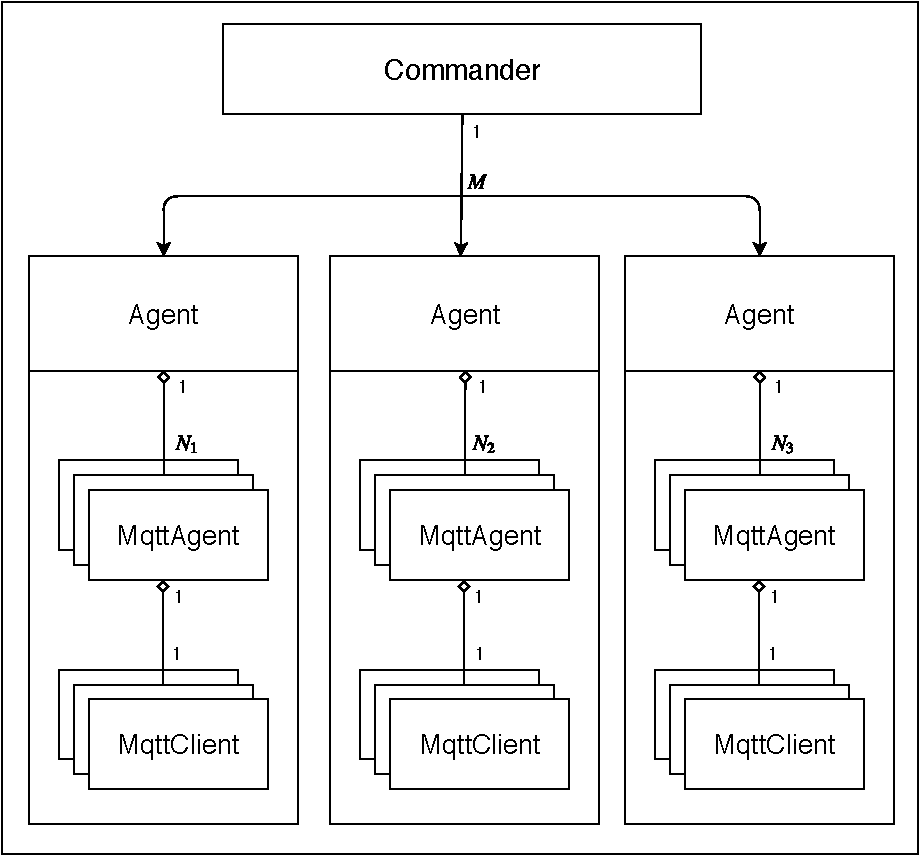
\includegraphics[scale=0.65]{Resources/PDF/Architecture}
	\caption{Varroa Distributed System Architecture}
	\label{pic:Architecture}
	\end{center}
\end{figure}
A Varroa Distributed System is composed of a Commander and multiple Agents.
The Commander and all Agents are executed in separate Varroa Instances.
Every Agent holds a number of MQTT Agents and each MQTT Agent manages one MQTT Client.
\newpage

\section{Commander}
\begin{figure}[h]
	\begin{center}
	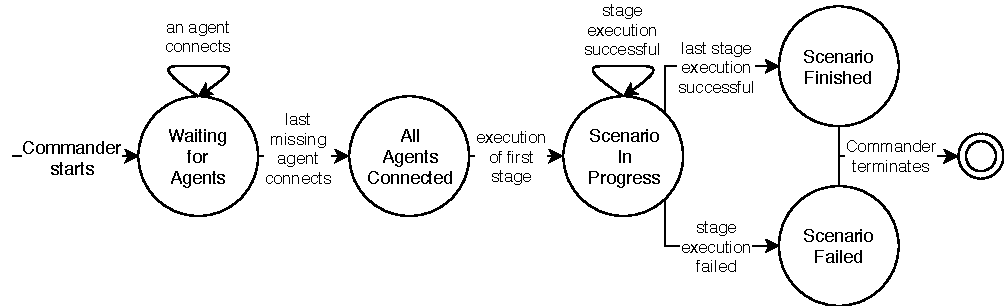
\includegraphics[scale=1]{Resources/PDF/CommanderStates}
	\caption{Commander States}
	\label{pic:CommanderStates}
	\end{center}
\end{figure}

\section{Chunk Distribution}
\begin{figure}[h]
	\begin{center}
	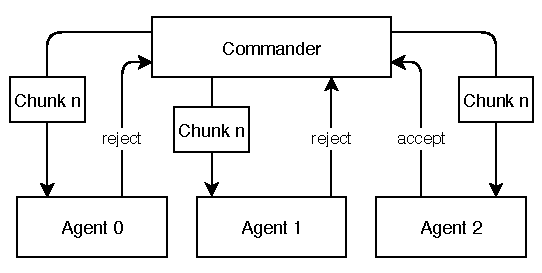
\includegraphics[scale=1]{Resources/PDF/ChunkDistribution}
	\caption{Distribution of a Chunk}
	\label{pic:ChunkDistribution}
	\end{center}
\end{figure}

\section{Chunk Handshake}
\begin{figure}[h]
	\begin{center}
	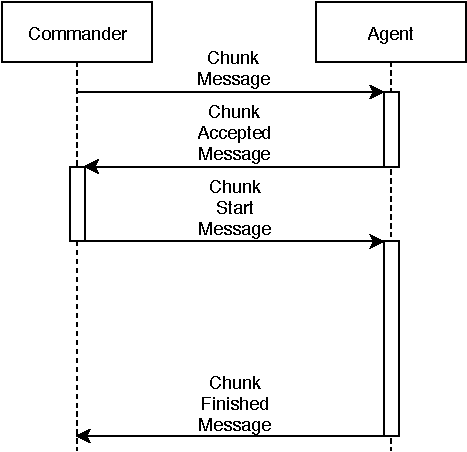
\includegraphics[scale=1]{Resources/PDF/ChunkAcceptedHandshake}
	\caption{Chunk Handshake with Accept}
	\label{pic:ChunkAcceptedHandshake}
	\end{center}
\end{figure}

\begin{figure}[h]
	\begin{center}
	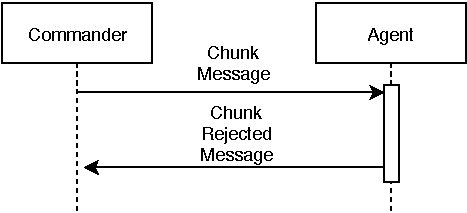
\includegraphics[scale=1]{Resources/PDF/ChunkRejectHandshake}
	\caption{Chunk Handshake with Reject}
	\label{pic:ChunkRejectHandshake}
	\end{center}
\end{figure}


% Abbildungsverzeichnis generieren.
\clearpage
\addcontentsline{toc}{chapter}{\listfigurename}
\listoffigures

% Tabellenverzeichnis generieren.
\clearpage
\addcontentsline{toc}{chapter}{\listtablename}
\listoftables

% Listingverzeichnis generieren.
%\clearpage
%\renewcommand{\lstlistlistingname}{Listingverzeichnis}
%\addcontentsline{toc}{chapter}{\lstlistlistingname}
%\lstlistoflistings

\end{document}
